\chapter{Introduction}

% Interest in building languages

Many kinds of programmers are interested in building new languages. General-purpose languages evolve slowly, but even so a dominant language like Java undergoes change over the years, adding new concepts and syntax \cite{java-generics}. New computer architectures spawn new languages \cite{ctm}\cite{cuda}\cite{opencl}, software engineers talk about how and when to build and use Domain Specific Languages \cite{fowler}, and of course programming language researchers are continually designing new languages to use or to analyze. Yet the technology that is currently used to construct programming languages does not support these kinds of creative activities very well, and often the lack of good tool support is a major factor discouraging the creation and use of a new language.

The design and implementation of languages, undertaken by a relatively small group of ``language vendors,'' is often seen as a separate task from the creation of programs by the much larger population of language users \cite{intentional}\cite{ward}. However, another approach, often identified with the Lisp community, views the task of writing a program as combined with the building of a language into one activity \cite{on-lisp}. These two perspectives go along with different tool sets, and the large disparity in goals suggests an opportunity exists to combine some of the strengths of both approaches in a single environment.

Furthermore, computer language technology could potentially be used in many more contexts. For instance, any class of structured documents (say recipes, essays, math problems) could be represented with a language defining the required elements and their relationships to each other. The tools used to create these documents are often far more user-friendly and visually rich than programming tools, but they fail to identify the underlying structure of the documents, trapping the data in a panoply of closed formats which obscure the valuable content. If the tools programmers use to create and work with languages offered better expressivity and were simpler to employ, software for creating many kind of documents could be built on similar foundations. 

%
% Previous approaches
%
\section{Existing Approaches}

\begin{figure}[h]
  \centering
  
%  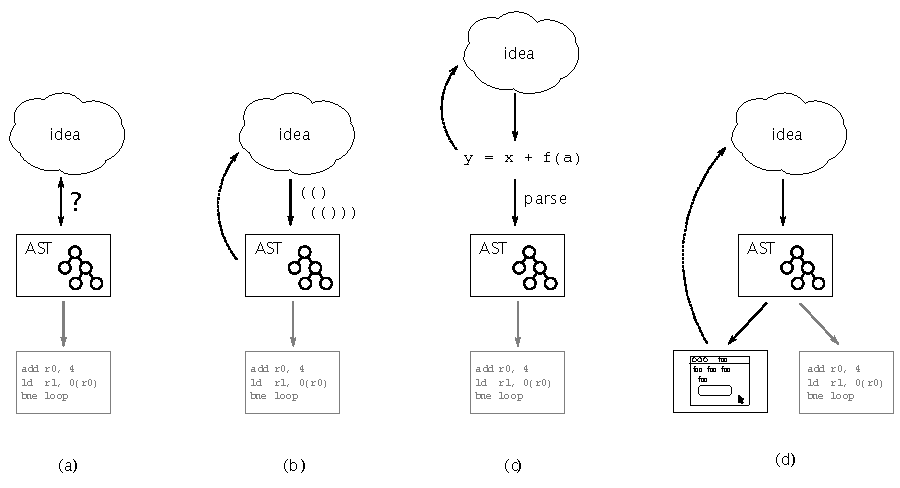
\includegraphics{src/image/figure1.pdf}

  \caption{The problem of turning an idea into a program, and three different solutions.}
  \label{fig-1}
\end{figure}

Figure \ref{fig-1}(a) illustrates the basic situation. A programmer has an idea for a program she wants her computer to run. To accomplish that, she needs to put the image in her mind into a form that can be understood by her computer. Since the advent of structured programming, virtually all programming languages have represented programs in terms of computational constructs arranged into a hierarchical structure. This tree-shaped structure, often called an Abstract Syntax Tree (AST), allows an infinite variety of programs to be constructed out of a small, fixed number of constructs, and provides an unambiguous representation for programs which can be consumed by tools such as compilers and interpreters. The programmer, on the other hand, may or may not think of her program in this way, and in any case she must translate the idea in her head into an AST, and then in a separate effort construct that AST within the memory of her computer.

Figure \ref{fig-1}(b) shows the simplest solution. The programmer describes the AST directly in a form that requires little or no interpretation. For example, she can write a Lisp program in s-expressions, using parentheses to explicitly indicate the nested structure of her program. In doing so, she actually engages in a process of action and feedback. She types a bit, perhaps attempts to run the program, reviews the program's source text (really only a thinly-veiled AST), and then elaborates on or revises the program. The programmer is able to inspect the AST almost directly, but has to do so by counting parentheses (dashed arrows in the figure show the path of feedback from the computer to the programmer).

These languages are easy to extend because introducing a new construct is accomplished by simply defining a new symbol, but the extra effort required to read them is off-putting to the overwhelming majority of programmers. This has lead to a decades-long cycle of proposals to ``fix'' the syntax and counter-argument \cite{lisp-hated}.

Instead, the majority use the model diagrammed in Figure \ref{fig-1}(c), where another representation stands between the programmer and the AST. Now she enters her program as free-form text, which is interpreted by a parser as directions for constructing the AST. This allows for a more ``natural''-appearing syntax, but it also inserts a level of indirection between the programmer and her program. The feedback loop of idea to program and back now goes from mind to \emph{text} and back, without ever involving the AST. In fact, the AST is now a mere by-product of the source text. 

The parser imposes both limits and costs. Because the textual syntax acts as both interface and specification, a tension is created between economy of expression (to serve the needs of the programmer) and precision (to allow a parser to construct the right AST). An economical syntax will often involve local ambiguity, because leaving some things unsaid which can be inferred from context is a hallmark of human communication. Furthermore, if language extension is to be an integral part of the construction of software, it is inevitable that different programmers working on different parts of a system will create language elements that are superficially similar, and that other programmers will need to combine these elements together.

In the presence of these ambiguities, parsers have to become context-sensitive to some extent. One solution is a custom parser---such as those commonly used to parse languages like Java and C---which is designed to handle a particular language and not easily extended. Therefore, these languages tend to provide a single fixed syntax and the cost to change it is very high---you may have to convince a standards body to incorporate your idea, and then wait for compiler vendors to implement it. The other is a more sophisticated parsing algorithm, which may be able handle local ambiguity, but the design of such parsers is an ongoing research problem, with significant performance costs \cite{frost}. 

A third approach is \emph{structure editing}. In Figure \ref{fig-1}(d), the programmer operates on the AST, with both presentation and editing mediated by an interface which explicitly understands the structure of the language. The first advantage of this setup is that the program's source is represented in the form of an AST, is edited at the level of the AST, and is always presented back to the user in terms of meaningful AST nodes. It's no longer possible for the programmer to \emph{read} the program one way while the parser disagrees. Secondly, the visual representation of the program---as well as the programmer's method of interacting with it---are not constrained to lines of text. The editor is free to supply more sophisticated layout, rendering, and forms of interaction.

Yet this power comes at a high cost. To construct a structure editor for a complete language is a large effort which may or may not justify its cost \cite{lang}. Worse still, structure editors are too specialized and too limiting to be embraced by real working programmers, who have accepted the weaknesses of the parser-driven approach and have grown dependent on a universe of text-based tools. Thus structure editors find use only in certain niches, where the benefits outweigh the perceived costs (e.g. end-user programming, CS education) \cite{alice}.

%
% My solution
%
\section{A New Way}

Each of the three approaches just described makes a fundamental trade-off between the conflicting goals of readability, expressive power, and extensibility. This thesis strikes a new balance, showing that by giving up textual source code, a new way of building languages can combine the expressive power of Lisp with the best syntax you can devise. I present a unified framework for constructing languages, editors, and compilers based on two simple ideas: all source code and derived objects are represented from the start as ASTs, and source is transformed into derived trees via reductions written in a simple, extensible, functional, meta-language.

\begin{figure}[th]
  \centering

%  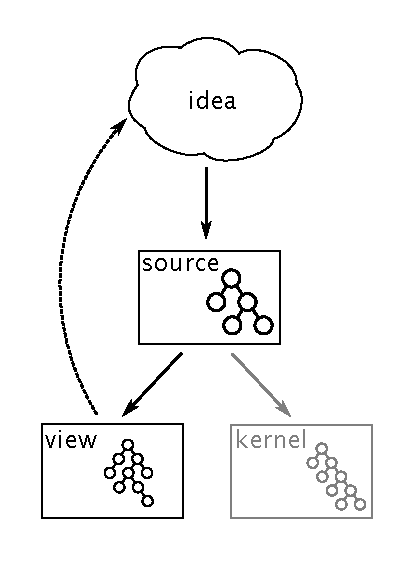
\includegraphics[scale=0.75]{src/image/figure2.pdf}

  \caption{\Meta}
  \label{fig-2}
\end{figure}

Figure \ref{fig-2} shows the high-level structure of \Meta's editing and execution model. Both the executable form of a program and its visual representation are defined in terms of ASTs (labeled \emph{kernel} and \emph{view}). The translation from the source form to these derived forms is specified in a modular way, with the same tools used to construct core languages and extensions. The programmer operates on the source AST in a relatively direct way, but this interaction is mediated by the ``view'' transformation, which presents the program in a familiar and understandable form.

The benefits of this approach are:

\begin{enumerate}

\item When constructed this way, a structure editor can be flexible enough to work with programs in multiple languages constructed in a dynamic process and freely embedded within one another.

\item Defining new language constructs or even entirely new languages is as simple as writing a program in an existing language, and the resulting languages are fully supported by the editing environment. Thus the barrier to entry for creating new languages is significantly reduced, and this approach may become a more routine part of the process of writing programs.

\item Freed from the constraints of parsing, more sophisticated presentation becomes easy to achieve. The tools prototyped so far can achieve excellent readability for typical programming constructs, but also support rich, familiar, mathematical notation.

\end{enumerate}

%
% Related Work
%
\section{Related Work}

% Structure editors:
Two recent projects have some of the same goals, and share the fundamental idea of moving to a tree-based representation for source code. Intentional Software is working on a tool based on Charles Simonyi's Intentional Programming work from the 1990s \cite{simonyi}, but little detail has been made public \cite{intentional}. The system appears to be targeted to large teams made up of \emph{domain experts} who are knowledgable in some field, and \emph{domain engineers} who are expert programmers, tasked with developing languages for the domain experts to use. Despite the difference in specifics, the Intentional Programming manifesto from 1995 aligns well with the assumptions and ideals of this thesis.

The Meta Programming System (MPS) \cite{mps}, from JetBrains, is a semi-proprietary product, which seems to be aimed more at programmers building languages for their own use or for the use of other programmers. MPS is based on an object-oriented approach to nodes and generation of (Java) code from the tree-structured source. Its editor and presentation language seem to be limited to mimicking the appearance and interaction style of textual source.

Both these systems seek to provide a complete environment for producing software (a Language Workbench \cite{workbench}), displacing the conventional tools, and consequently they are multi-person-year projects. This thesis aims to show that useful functionality is possible with just a small, compact system.

MetaEdit \cite{metaedit} is a commercial system aimed at (non-textual) modeling languages. Tools addressing the difficulty of implementing good tool support for textual DLS are many, often targeting the free Eclipse IDE platform: \cite{xtext}\cite{spoofax}\cite{stratego}. 

Structure editors, or syntax-directed editors, had their greatest flowering in the 1980s, but usually had very different goals, including improved compiler performance (via incremental compilation) \cite{cps}\cite{zavodnik}. Lang provides an interesting retrospective \cite{lang}.

Barista \cite{barista}, built on Citrus \cite{citrus}, is a more recent structure editor for Java exploring new user interface paradigms for editing code.

% notational richness:
The Fortress language~\cite{fortress} has similar aspirations with regard to the faithful reproduction of mathematical notation. Indeed its creator cites improved notation as one of three key ideas for the language~\cite{fortress-parallel}. It supports the use of any Unicode~\cite{unicode} symbol as an operator. However, Fortress's primary source format is ordinary text; programs are typically written in text and then translated to a richer presentation (via \TeX) for publishing. This approach harks all the way back to Algol 60's multiple languages, and even the never-implemented m-expressions of Lisp. The Fortress spec also includes a mechanism for syntax extension, but it does not appear to have been implemented.

%\todo{really an example more then related work?}Even modest extensions to existing languages typically require new tools. Sikuli is a user-interface scripting language which adds one construct to ordinary Python syntax: embedded screenshots. The source code is Python with string literals referring to files containing image data, and ``Sikuli IDE integrates screen capturing and a custom text editor''\cite{sikuli}, replacing paths with the actual images. Scripts are executed using a regular Python interpreter (Jython), augmented by an image-processing library. To use this language as intended, one has to abandon whatever editor one uses for all other programming tasks and adopt this new tool.


% summary

I present a representation for ASTs and fundamental tools for manipulating them in Chapter~\ref{ASTs}. Chapter~\ref{languages} shows how languages are defined and extended. Chapter~\ref{prototype} describes the prototyped system which implements these ideas, and Chapter~\ref{studies} presents two case studies of the effectiveness of the system for defining new syntax and programming constructs. 


